%%%%%%%%%%%%%%%%%%%%%%%%%%%%%%%%%%%%%%%%%
% Imperial College London Poster (Landscape)
% LaTeX Template
% Version 1.0 (February 22, 2024)
%
% For current versions and to report
% issues, please see:
% https://github.com/ImperialCollegeLondon/imperial_latex_templates
%
%!TEX program = xelatex
% Note: this template must be compiled with XeLaTeX rather than PDFLaTeX
% due to the custom fonts used. The line above should ensure this happens
% automatically, but if it doesn't, your LaTeX editor should have a simple toggle
% to switch to using XeLaTeX.
%
% © Imperial College London, 2024. This template, including logo and fonts, is 
% for use of Imperial staff and students only for university business. All rights 
% reserved to the copyright owners.
%
%%%%%%%%%%%%%%%%%%%%%%%%%%%%%%%%%%%%%%%%%

%----------------------------------------------------------------------------------------
%	CLASS, PACKAGES AND OTHER DOCUMENT CONFIGURATIONS
%----------------------------------------------------------------------------------------

\documentclass[
	landscape, % Landscape page orientation
	%print, % Uncomment to convert colors to CMYK for printing purposes
	%a1papersize, % Uncomment to use an A1 paper size instead of the default A0 paper size
]{ImperialPoster}
\usepackage{amsmath}
\usepackage{amssymb}
\usepackage{algpseudocode}
\usepackage{algorithm}
%----------------------------------------------------------------------------------------
%	POSTER INFORMATION
%----------------------------------------------------------------------------------------

\postertitle{Learning to Bid Above a Threshold Using Multi-Armed Bandits} % The poster title, can be split across multiple lines manually with \\

% Contributor/author names, can be split across multiple lines manually with \\
% Add affiliations using the \affiliation{} command
\posterauthors{Quentin Leconte,\\ Supervisor: Ciara Pike-Burke}

% Command to output coauthor logos to the right of the Imperial logo in the header of the poster
% If no coauthor logos are required, remove or comment out this command
% \coauthorlogos{
% 	\coauthorlogo[4cm]{Grey_16-9.pdf} % Use the optional parameter to specify a height for the logo
% 	\coauthorlogo[4cm]{Grey_16-9.pdf} % Use the optional parameter to specify a height for the logo
% 	\coauthorlogo{Grey_16-9.pdf} % Not specifying the optional parameter will make the logo the same height as the Imperial logo
% }

%----------------------------------------------------------------------------------------

\begin{document}

%----------------------------------------------------------------------------------------
%	EXAMPLE POSTER LAYOUT 1
%----------------------------------------------------------------------------------------

\titlesection % Output the title section, automatically populated using the information in the POSTER INFORMATION block above

\medskip % Vertical whitespace

\begin{multicols}{4} % Start the four-column layout
	
	%----------------------------------------------------------------------------------------
	%	FIRST COLUMN
	%----------------------------------------------------------------------------------------
	
	\subsection{1. Problem}
	\textcolor{ICLBlue}{Situation:} \textit{During an auction, $T$ products are offered one after the other. A \textcolor{ICLBlue}{threshold} $\tau_t$ is associated with each product, for round $t = 1, \dots T$. 
	Only one \textcolor{ICLBlue}{bid} $b_t$ can be made per round, and the product is won if it is above the threshold Figure \ref{fig:bid_threshold}. How can the number of products won be maximised while minimising the value of the bids?}\\
	\begin{figure}[H] % [H] forces the figure to be output where it is defined in the code (it suppresses floating)
		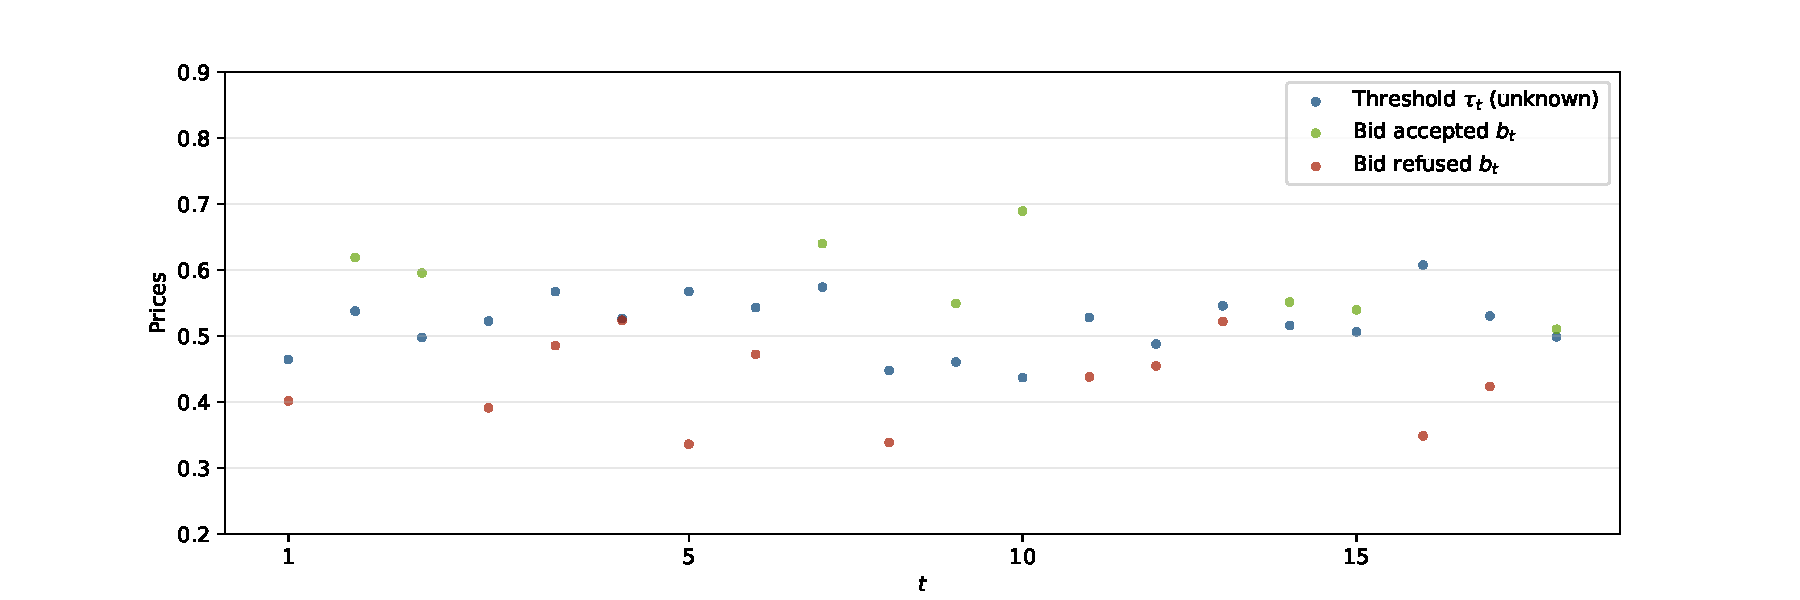
\includegraphics[width=\linewidth]{"../../../../figures/bid_threshold.pdf"} % Figure image
		\caption{Acceptance and rejection of bids $b_t$ based on thresholds $\tau_t$.}
		\label{fig:bid_threshold}
	\end{figure}
	\begin{itemize}
		\item The bid values and thresholds range between 0 and 1.
		\item The thresholds are i.i.d and $\tau_t \sim \mathcal{N}(\tau, \sigma^2)$, unknown parameters.
		\item Only the information $\delta_{t} = \mathbb{I}_{\{b_{t} \geq \tau_{t}\}}$ is known after making the bid $b_t$.
		\item The interval $[0,1]$ is \textcolor{ICLBlue}{partitioned} into $J$ sub-intervals of equal size. Playing \textcolor{ICLBlue}{arm} $j$ at round $t$ is then equivalent to making a bid 
		$b_t^{(j)}$ uniformly in $\left[a_0^{(j)}, a_1^{(j)}\right],$ where $a_0^{(j)} = \frac{j-1}{J}$ and $a_1^{(j)} = \frac{j}{J}$.
		\item The \textcolor{ICLBlue}{reward} associated with each round (after playing arm $j$) is
		$$X_t^{(j)} = \delta_t^{(j)} (b_{\sup} - b_t^{(j)}).$$
	\end{itemize}
    \subsection{2. Strategies for Selecting the Arm to Maximise Reward}
	
	\begin{itemize}
		\item For each arm $j$, the \textcolor{ICLBlue}{expected reward} (independent of $t$) $\mu_j = \mathbb{E}\left[X^{(j)}|\tau, \sigma\right]$, given the parameters of the threshold distribution, can be calculated. The expected rewards are plotted for 
		$J = 1000$ and some values of $\tau$ and $\sigma$ in Figure \ref{fig:exp_rew}.
	\end{itemize}

	\begin{figure}[H] % [H] forces the figure to be output where it is defined in the code (it suppresses floating)
		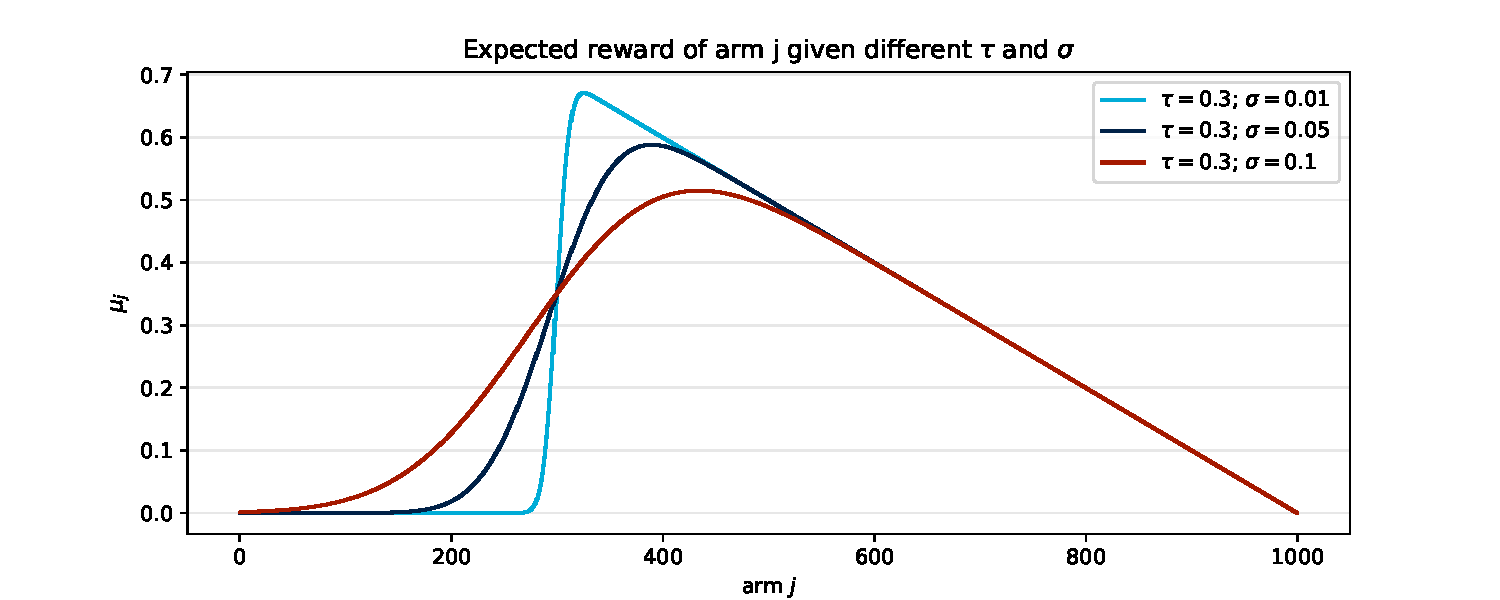
\includegraphics[width=\linewidth]{"../../../../figures/expect_rew.pdf"} % Figure image
		\caption{Barplots of expected rewards for 1000 arms partitioning $[0,1]$ for different threshold distribution generated from $\mathcal{N}(\tau, \sigma^2)$ ($\tau = 0.3$ and $\sigma \in \{0.01, 0.05, 0.1\}$).
		The smaller $\sigma$ is, the closer the optimal arm is to $\tau \times J$.}
		\label{fig:exp_rew}
	\end{figure}
	\begin{itemize}
		\item After playing arm $j$, the \textcolor{ICLBlue}{empirical expected reward} 
		$$\hat{\mu}^{(j)}_t = \frac{1}{\max\left(1,N_j(t)\right)}\sum_{s=1}^{t} X_{s}^{(j)} \mathbb{I}_{\{J_s = j\}}$$ is updated, where $J_s$ is the 
		arm played in round $s$ and $N_j(t) = \sum_{s=1}^{t}\mathbb{I}_{\{J_s = j\}}$.
	\end{itemize}

	\subsection{3. Algorithm}
	
	\begin{itemize}
		\item The approach presented is strongly inspired by the \textcolor{ICLBlue}{sequential halving algorithm}\cite{SHA}. As shown in Figure \ref{fig:exp_rew}, the function
		$j \rightarrow \mu_j$ is a step function with a single maximum. The algorithm is divided into episodes of three rounds and aims to find an increasingly precise bracket for the optimal arm $j^*$
		in each episode. At each episode, a left arm, middle arm, and right arm are repeatedly assigned to get as close as possible to the optimal arm.
		The assignment of arms is described in Algorithm \ref{alg:SHA} and illustrated in Figure \ref{fig:new_arms}.
	\end{itemize}

	\begin{algorithm}[H]
		\caption{Adapted Sequential Halving Algorithm}\label{alg:SHA}
	    \begin{algorithmic}
		\State \textbf{Input:} $n_{ep}$ \Comment{number of times an arm is played per episode.}
		\State \textbf{Initialize:} Episode 0: $L, M, R \gets1,\lfloor K/2 \rfloor,  K$;
		\For{Episode = 1, \dots}
		\State \textbf{Play} each arm $n_{ep}$ times
		\State $t_{ep}$ is the final round number of episode
		\If{$\hat{\mu}_{t_{ep}}^{L} < \hat{\mu}_{t_{ep}}^{M}$ and $\hat{\mu}_{t_{ep}}^{R}< \hat{\mu}_{t_{ep}}^{M}:$}
			\State $L, M, R \gets \lfloor (L + M)/2\rfloor, M, (R + M)/2$
		\EndIf
		\If{$\hat{\mu}_{t_{ep}}^{L} < \hat{\mu}_{t_{ep}}^{M} < \hat{\mu}_{t_{ep}}^{R}:$}
			\State $L, M, R \gets M, R, 2R - M$
		\EndIf
		\If{$\hat{\mu}_{t_{ep}}^{L} > \hat{\mu}_{t_{ep}}^{M} > \hat{\mu}_{t_{ep}}^{R}:$}
			\State $L, M, R \gets 2 L - M, L, M$
		\EndIf \Comment{Certain cases must be handled differently when the boundary arms are reached.}
		\EndFor
	     \end{algorithmic}
		\end{algorithm}

	\begin{figure}[H] % [H] forces the figure to be output where it is defined in the code (it suppresses floating)
		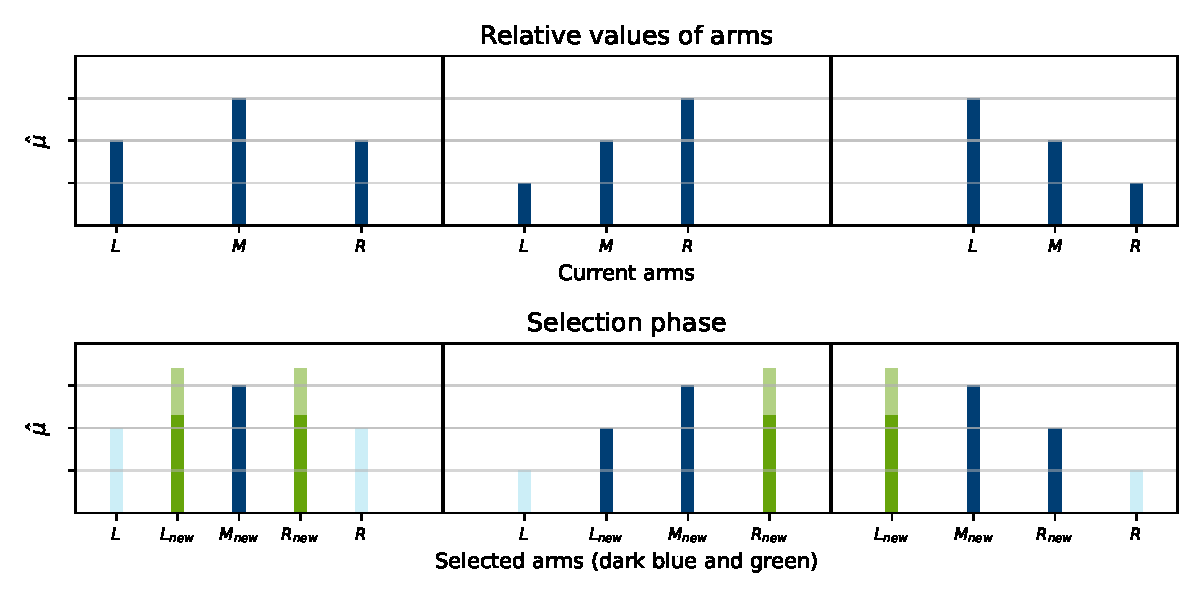
\includegraphics[width=\linewidth]{"../../../../figures/arm_assignment.pdf"} % Figure image
		\caption{Selection of new left, middle, and right arms based on the empirical expected reward relative values of the current left, middle, and right arms.}
		\label{fig:new_arms}
	\end{figure}
	\begin{itemize}
		\item The \textcolor{ICLBlue}{regret} of an algorithm over $t$ rounds is
		$$\mathfrak{R}_t(\pi) = \sum_{s=1}^{t}(\mu^* - \mu_{J_s}),$$
		where $\mu^* = \max_{j = 1, \dots J}\mu_j$ is the expected reward of the optimal arm. The algorithms aim to minimise their regret.
		Two examples of regret plots are in Figure \ref{fig:regret}.
	\end{itemize}
	\begin{figure}[H] % [H] forces the figure to be output where it is defined in the code (it suppresses floating)
		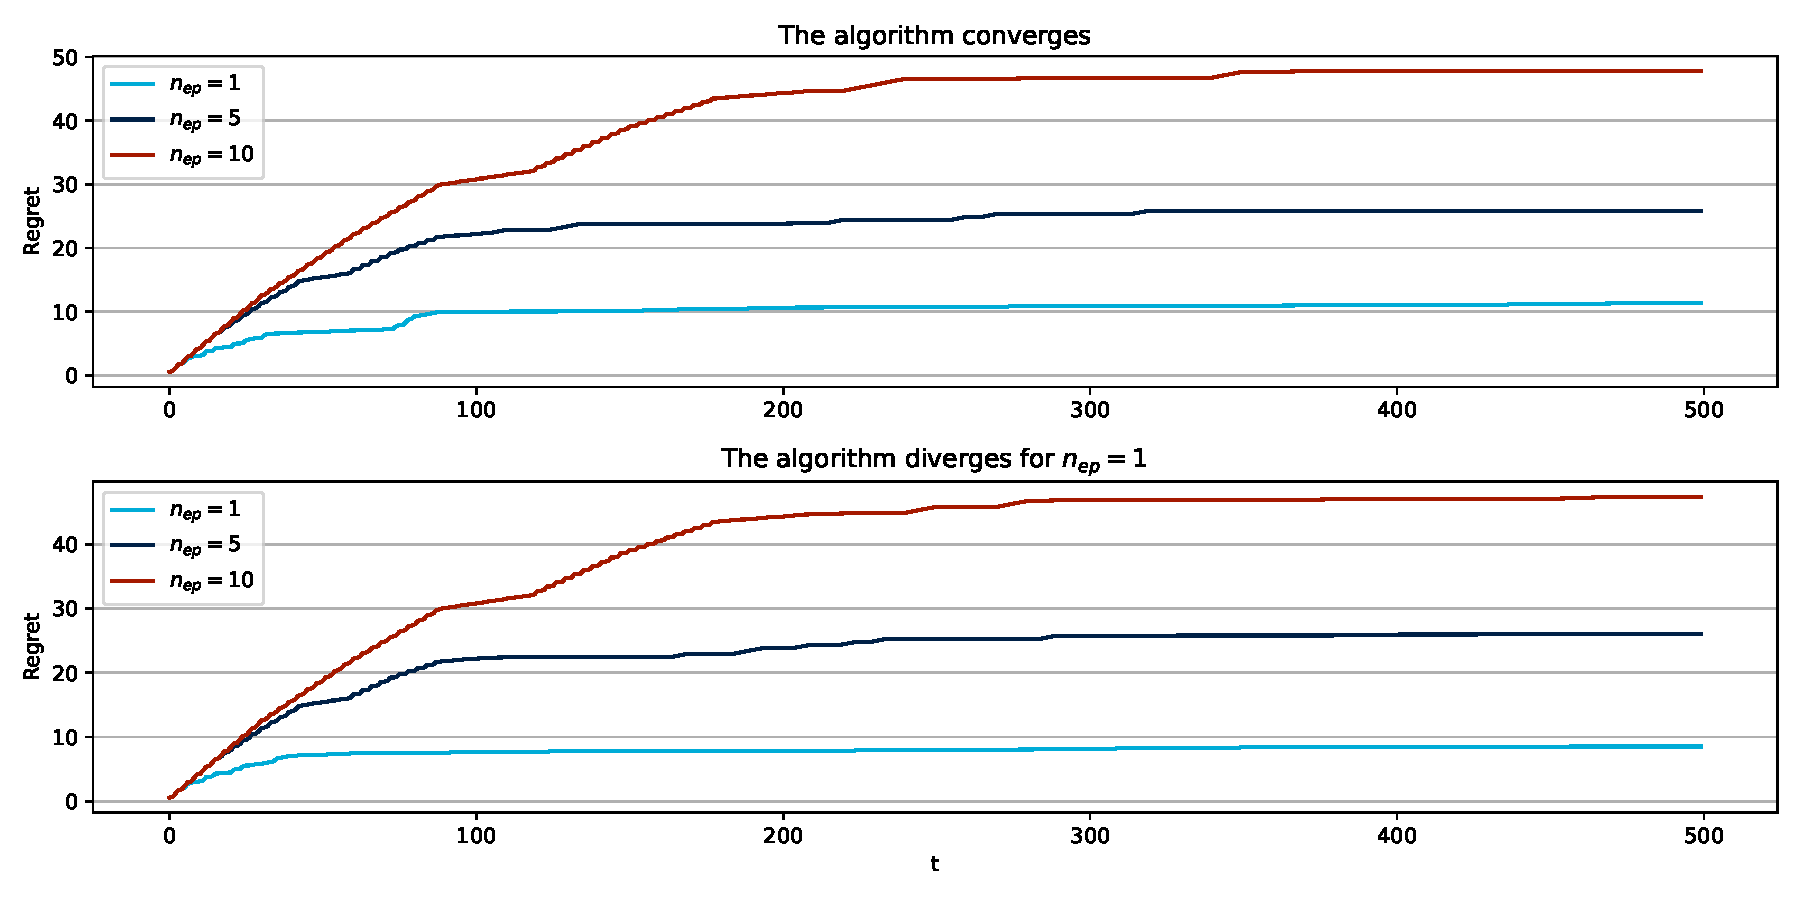
\includegraphics[width=\linewidth]{"../../../../figures/regret.pdf"} % Figure image
		\caption{Regret plot of adapted sequential halving theorem for $K = 50$, $\tau = 0.4$, $\sigma = 0.01$. Several simulations were done until convergence or divergence. The algorithm is not stable, especially when $n_{ep}$ is low.}
		\label{fig:regret}
	\end{figure}

	% \subsection{Using EM algorithm}

	% For $t_0, t_1 \in \{1, \dots T\}$ and $t_0 < t_1$, the set $(\delta_s)_{s = t_0}^{t_1}$ corresponds to left and right censored data. The EM algorithm can then be used to estimate 
	% the parameters $\tau$ and $\sigma$ of the threshold distribution. Arm $j^* = \text{argmax}_{j = 1, \dots J}\mathbb{E}\left[X^{(j)}| \hat{\tau}, \hat{\sigma}\right]$ is chosen.
	% A strategy must be found to divide the set of rounds into episodes, each having a starting round $t_0$ and an ending round $t_1$.
 

	\begin{thebibliography}{5}
		\bibitem{SHA}
		Cheshire, James and Menard, Pierre and Carpentier, Alexandra (2021) \emph{Problem Dependent View on Structured Thresholding Bandit Problems, Proceedings of the 38th International Conference on Machine Learning, p1846--1854}
		\end{thebibliography}
\end{multicols}

%----------------------------------------------------------------------------------------
%	EXAMPLE POSTER LAYOUT 2
%----------------------------------------------------------------------------------------

% \newpage

% \titlesection % Output the title section, automatically populated using the information in the POSTER INFORMATION block above

% \medskip % Vertical whitespace

% \begin{multicols}{4} % Start the three-column layout
	
% 	%----------------------------------------------------------------------------------------
% 	%	FIRST COLUMN
% 	%----------------------------------------------------------------------------------------
	
% 	\subsection{Subsection Title}
	
% 	Adi cum fugia qui dolo ommodit quia venisi saperat iscim qsequae nobissitat.
	
% 	Sed que perspic ipsanihit quunt aligenist re reperehendia \textcolor{ICLBlue}{apicias re pellectur sustentur?}
	
% 	Ehendios \textcolor{ICLBlue}{dolores} ni dolut acero del mint apid esto bernatendem eum \textcolor{ICLBlue}{atqui delisti opta} aliquam il id quam fuguist, eum rerferesto conserro berionectio. Alitatu saperat iscim qsequae.
	
% 	\begin{quote}
% 	"Pull Quote/Subtitle. Oluptat ut in gother comnihic totatem apietur, ium audi imus vent ipsum volup ta veniscil dolut acero del mint conserro"
% 	\end{quote}
	
% 	\subsection{Subsection Title}
	
% 	Adi cum fugia qui dolo ommodit quia venisi saperat iscim qsequae nobissitat.
	
% 	Sed que perspic ipsanihit quunt aligenist re reperehendia apicias re pellectur sus, tentur? 
	
% 	\begin{table}[H] % [H] forces the table to be output where it is defined in the code (it suppresses floating)
% 		\caption{Experimental results.}
% 		\begin{tabular}{L{0.24\linewidth} C{0.24\linewidth} R{0.24\linewidth}}
% 			\toprule
% 			Treatment & Quantity & Response\\
% 			\midrule
% 			AAA & 10mL & 0.944\\
% 			AAA & 150mL & 0.527\\
% 			BBB & 20mL & 0.263\\
% 			BBB & 2,000mL & 0.818\\
% 			\bottomrule
% 		\end{tabular}
% 	\end{table}
	
% 	\columnbreak % Switch to the next column
	
% 	%----------------------------------------------------------------------------------------
% 	%	SECOND COLUMN
% 	%----------------------------------------------------------------------------------------
	
% 	\section{Section Title}
	
% 	Equae es nobissitat hitatum estis quodit larib ustotatet etur aut exere estint eium ium expeb usantis sae maio omnis consed quam reici voluptam ipistio. Arum, se velliquosam, oms evelendici derroruptius debitis quunto. 
	
% 	\smalltext{Equae es nobissitat hitatum estis quodit larib ustotatet etur aut exere estint eium ium expeb usantis sae maio omnis consed quam reici voluptam ipistio.} % Use \smalltext or an enclosed \small for a block of text in a reduced font size
	
% 	\begin{figure}[H] % [H] forces the figure to be output where it is defined in the code (it suppresses floating)
% 		
\includegraphics[width=0.495\textwidth]{Grey_4-3.pdf} % Figure image
% 		\parbox[b]{0.495\textwidth}{\caption{Lorem ipsum dolor sit amet, consectetur adipiscing elit. Praesent porttitor arcu luctus, imperdiet urna iaculis, mattis eros.}} % Caption needs to be in a parbox of the same width as the figure in order to span the same width across 2 columns
% 	\end{figure}
	
% 	\columnbreak % Switch to the next column
	
% 	%----------------------------------------------------------------------------------------
% 	%	THIRD COLUMN
% 	%----------------------------------------------------------------------------------------
	
% 	\begin{figure}[H] % [H] forces the figure to be output where it is defined in the code (it suppresses floating)
% 		
\includegraphics[width=\linewidth]{Grey_16-9.pdf} % Figure image
% 		\caption{Figure caption. Lorem ipsum dolor sit amet, consectetur adipiscing elit. Praesent porttitor arcu luctus.}
% 	\end{figure}
		
% 	\columnbreak % Switch to the next column
	
% 	%----------------------------------------------------------------------------------------
% 	%	FOURTH COLUMN
% 	%----------------------------------------------------------------------------------------
	
% 	\section{Section Title}
	
% 	\begingroup
% 		\small % Reduce font size
% 		Obisim qui quiae porum ea volorenis eic tem andae nus, verem expligento tecum eos quo magnihit inis sunt di dolupta tiuntem qui ipid moluptatquam idio. Itinturia vellam in none velit quat landi ium faci dolum volut as ea cus.

% 		Am conet, ut occaerum ant eatibusdae sit, nus etur? Mincia cone verum qui dis nobitatur sequodi oriaepuda sim rempersperia nulluptatis culpario eicte illupta tenemperit isquamus natem.\par
% 	\endgroup
	
% 	\largepercent{95\%} % Large bold percentage figure
	
% 	\begin{enumerate}
% 		\item Lorem ipsum
% 		\item Lorem ipsum dolor sit amet, consectetur adipiscing elit.
% 		\item Praesent porttitor.*
% 	\end{enumerate}
	
% 	\smalltext{*Equae es nobissitat hitatum estis quodit laborib ustotatet e auexere estint eium ium experib usantis sae maio omnis co.} % Use \smalltext or an enclosed \small for a block of text in a reduced font size
		
% 	\boldsection{Arum alis dolum aut pe dolorestem cone verestis es si beaquib usanime eum} % Output some bold text to stand out from the body text
	
% 	Equae es nobissitat hitatum estis quodit larib ustotatet etur aut exerem ium exeb.
	
% 	\subsection{Affiliations}
	
% 	% Affiliation institutions, the first parameter is the affiliation number (matching the author list) and the second is the institution
% 	\affiliationentry{1}{Department Name, Imperial College London}\\
% 	\affiliationentry{2}{University Name}\\
% 	\affiliationentry{3}{Institute Name}
	
% 	\subsection{Funders}
	
% 	
\includegraphics[width=0.55\linewidth]{UKRI_logo.png}\hfill
\includegraphics[width=0.35\linewidth]{Grey_16-9.pdf} % Side by side funder logos
	
% %----------------------------------------------------------------------------------------

% \end{multicols}

% %----------------------------------------------------------------------------------------

\end{document}
